\section{Results}
\label{sec:results}

Through this section we discuss the experimental tests, along with the valuation strategy carried out. 

The main purpose of our test is to understand how many tags for each service 
are correctly addressed. In order to achieve this, we distributed GHio-Ca to 
30 testers and asked to de-select tags that did not concern shots that they 
have taken. Finally, they had to send the result to us.

Our approach was to make as simple as possible for the tester to contribute: 
we (i) made a video tutorial\footnote{\url{https://youtu.be/G9PSzpBI5LA}} in 
which we showed what they had to do, (ii) wrote a mini-wiki where the 
experiment was explained, (iii) modified the application. 

According to our planning, each testing member was asked to take 5 photos. 
The final number of photos that we received is 150.

\subsection{Tester vs Normal version}

We needed to implement three main changes to the normal version to be able to 
carry out the experiment. The first one is about the way we retrieved results 
from services: in the normal version, the tags are merged together, instead in 
the test version we did not merge them.
Abuse of APIs calls from users was our main concern. To solve this issue, we 
put a limit on the maximum number of pictures that a tester could take.
Last but not least is how the results are shared. With the test version, we 
only allowed users to share the content with e-mail applications, sending tags 
and photos to our hard-coded email address.

\subsection{Graphical analysis}

At the end of the testing phase, we collected all the e-mails received, we 
counted them and we built several graphical representations that we 
explain as follows.

\begin{figure}[htp]
\centering
    \subfloat[Azure tagging results (708 tags provided)]{
        \label{img:testgraphsazure}
        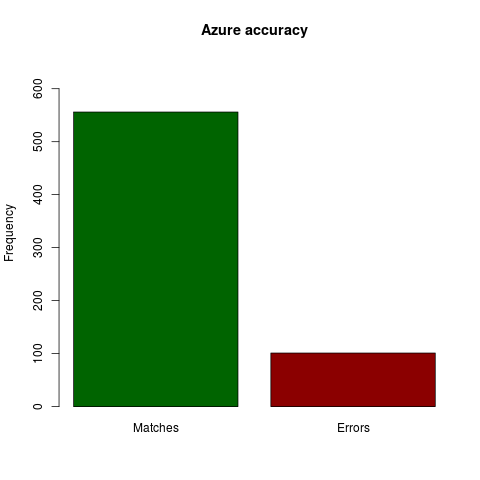
\includegraphics[width=0.45\linewidth]
        {AzureGraph}
    }
    \hfill
    \subfloat[Google tagging results (32 tags provided)]{
        \label{img:testgraphgoogle}
        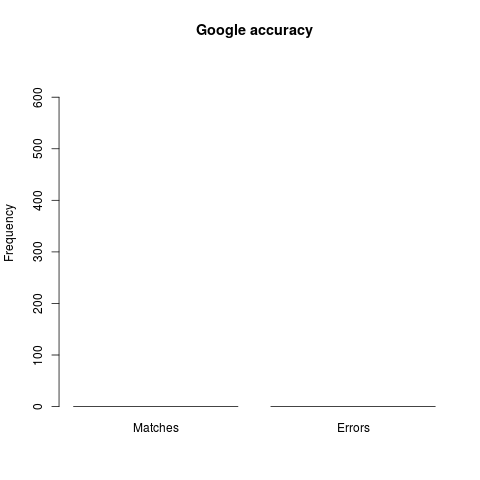
\includegraphics[width=0.45\linewidth]
        {GoogleGraph}
    }
    \\
    \subfloat[Imagga tagging results (520 tags provided)]{
        \label{img:testgraphimagga}
        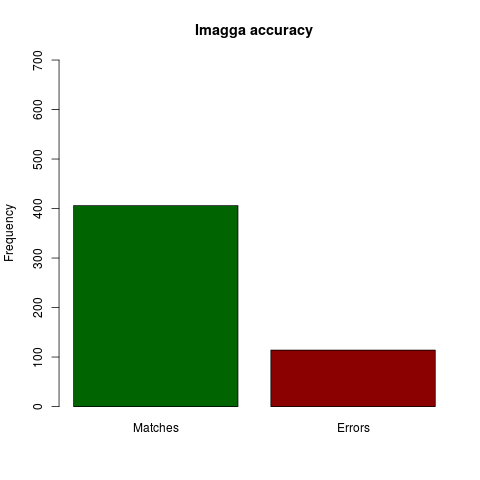
\includegraphics[width=0.45\linewidth]
        {ImaggaGraph}
    }
    \hfill
    \subfloat[Watson tagging results (841 tags provided)]{
        \label{img:testgraphwatson}
        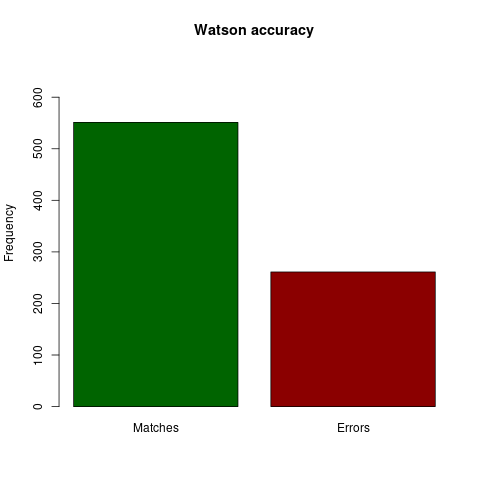
\includegraphics[width=0.45\linewidth]
        {WatsonGraph}
    }
    \caption{Frequencies histogram of matches / mismatches}
\end{figure}

In first place, Azure was the service that gave us the best results with 85\% 
of correct tags (Figure~\ref{img:testgraphsazure}), on the other hand Google 
Reverse Image Search (Figure~\ref{img:testgraphgoogle}) was the worst one (
with only 31\% of matches), but we have to advocate that it was not designed 
to provide tags from/to user images, thus we did not expect good results from 
this service.
Imagga (Figure~\ref{img:testgraphimagga}) and Watson 
(Figure~\ref{img:testgraphwatson}) (respectively a service we found online and 
an IBM Image Recognition service) didn't stand out as we expected: for the 
first one we had to filter a good chunk of tags since a lot of them had a low 
confidence of correlation with images and the second one provided a lot of 
tags that turned out to be wrong. The percentages of good tags are 78\% for 
Imagga and 65\% for IBM Watson.

\begin{figure}[H]
\centering
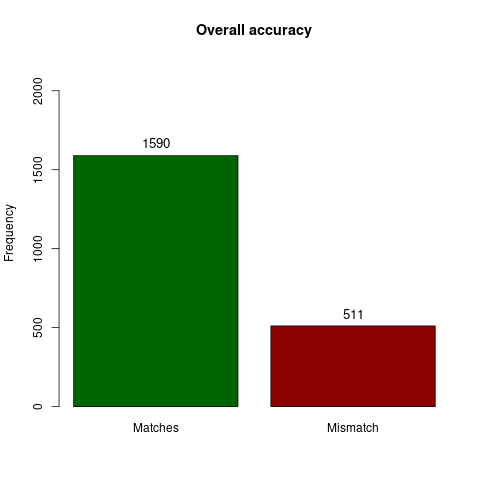
\includegraphics[scale=0.3]{OverallGraph}
\caption{Histogram of all tagging results (2101 tags provided)}
\label{img:testgraphoverall}
\end{figure}

In Figure~\ref{img:testgraphoverall} we can see the overall representation, 
with a percentage of 75\% of correct tags, that we consider to be a good 
result.

\begin{figure}[htp]
\centering
    \subfloat[Histogram of all searches that give back at least one match]{
        \label{img:testatleastone}
        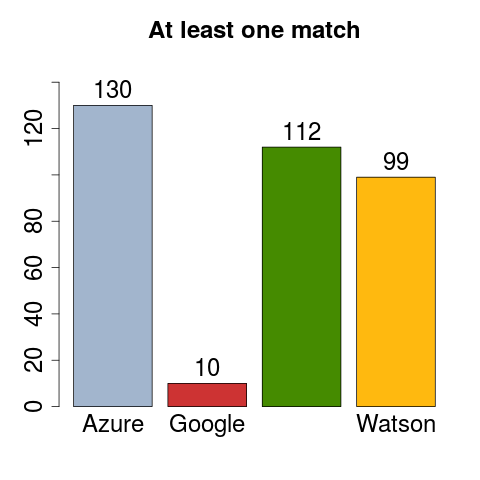
\includegraphics[width=0.45\linewidth]
        {AtLeastOneMatchGraph}
    }
    \hfill
    \subfloat[Histogram of all searches that give back only correct tags]{
        \label{img:testcompletematch}
        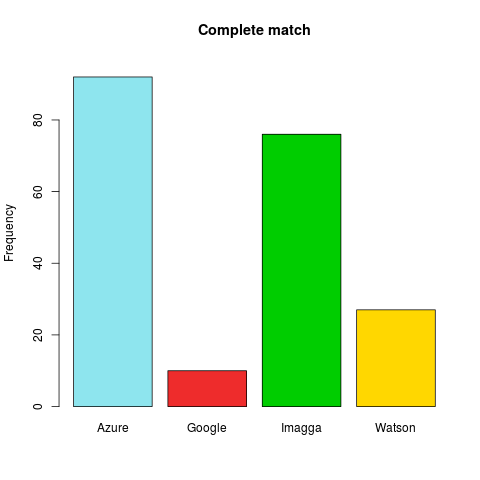
\includegraphics[width=0.45\linewidth]
        {CompleteMatchGraph}
    }
\end{figure}

In Figure~\ref{img:testatleastone} we can see the number of times that 
services gave back at least one correct tag. Even in this case, Azure was the 
service that had the best performance but also Watson and Imagga gave back 
results that are good enough.

Finally, we present in Figure~\ref{img:testcompletematch} the number of times 
that a service returned a bunch of tags that were all confirmed as matches by 
a user. In this case Azure and Imagga had the best results. In this case even 
Google Reverse Image Search has a positive result, because it gives to the user 
only one tag that could be accepted or not.

\subsection{Character recognition}

\begin{figure}[H]
\centering
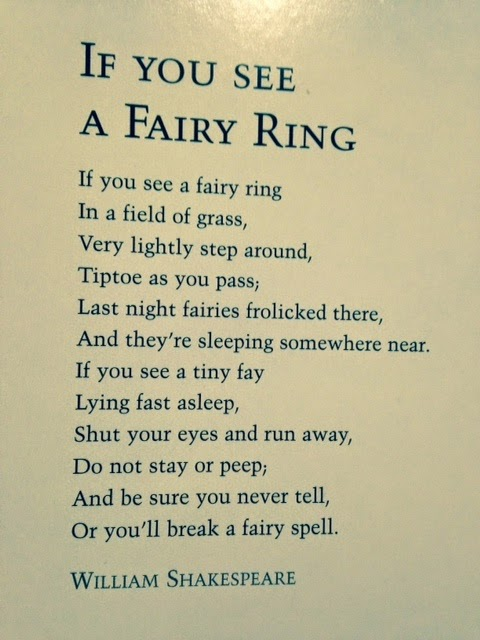
\includegraphics[scale=0.25]{ocr}
\caption{Example of photo with text}
\label{testOCR}
\end{figure}

Execution of OCR in Figure~\ref{testOCR} gives the following result:
\begin{lstlisting}
IF YOU SEE
A FAIRY RING
if you see a fairy ring
in a field of grass,
very lightly step around,
tiptoe as you pass;
last night fairies frolicked there,
and they're sleeping somewhere near.
if you see a tiny fay
lying fast asleep,
shut your eyes and run away,
do not stay or peep;
and be sure you never tell,
or you'll break a fairy spell.
WILLIAM SHAKESPEARE
\end{lstlisting}

In this case, we obtain a perfect match. However, with different resolutions 
of images and different languages, the results are not so good. Unfortunately, 
we were not able to gain enough data to build a good evaluation set.